\documentclass[twoside]{article}
\usepackage[a4paper]{geometry}
\geometry{verbose,tmargin=2.5cm,bmargin=2cm,lmargin=2cm,rmargin=2cm}
\usepackage{fancyhdr}
\pagestyle{fancy}

% nastavení pisma a~češtiny
\usepackage{lmodern}
\usepackage[T1]{fontenc}
\usepackage[utf8]{inputenc}
\usepackage[czech]{babel}

% odkazy
\usepackage{url}

\usepackage{float}
% vícesloupcové tabulky
\usepackage{multirow}
\usepackage{listings}
\usepackage{xcolor}
\usepackage{amssymb}
\usepackage{gensymb}
\usepackage{bbold}
\usepackage{amsmath}
\usepackage{siunitx}
\usepackage{mathtools}
\usepackage{commath}

% vnořené popisky obrázků
\usepackage{subcaption}

% automatická konverze EPS 
\usepackage{graphicx} 
\usepackage{epstopdf}
\epstopdfsetup{update}

\graphicspath{{./images}}

% odkazy a~záložky
\usepackage[unicode=true, bookmarks=true,bookmarksnumbered=true,
bookmarksopen=false, breaklinks=false,pdfborder={0 0 0},
pdfpagemode=UseNone,backref=false,colorlinks=true] {hyperref}


% Poznámky při překladu
\usepackage{xkeyval}	% Inline todonotes
\usepackage[textsize = footnotesize]{todonotes}
\presetkeys{todonotes}{inline}{}

%https://tex.stackexchange.com/questions/2783/bold-calligraphic-typeface
\DeclareMathAlphabet\mathbfcal{OMS}{cmsy}{b}{n}

% enumerate zacina s pismenem
\renewcommand{\theenumi}{\alph{enumi}}

% smaz aktualni page layout
\fancyhf{}
% zahlavi
\usepackage{titling}
\fancyhf[HC]{\thetitle}
\fancyhf[HLE,HRO]{\theauthor}
\fancyhf[HRE,HLO]{\today}
 %zapati
\fancyhf[FLE,FRO]{\thepage}

% údaje o autorovi
\title{OTE Domácí úkol 10 - Digitalizace a rekonstrukce signálu}
\author{Vojtěch Michal}
\date{\today}

%customize code listing
\definecolor{codegreen}{rgb}{0,0.6,0}
\definecolor{codegray}{rgb}{0.5,0.5,0.5}
\definecolor{codepurple}{rgb}{0.58,0,0.82}
\definecolor{backcolour}{rgb}{0.95,0.95,0.92}

\lstdefinestyle{mystyle}{
    backgroundcolor=\color{backcolour},   
    commentstyle=\color{codegreen},
    keywordstyle=\color{magenta},
    numberstyle=\tiny\color{codegray},
    stringstyle=\color{codepurple},
    basicstyle=\ttfamily\footnotesize,
    breakatwhitespace=false,         
    breaklines=true,                 
    captionpos=b,                    
    keepspaces=true,                 
    numbers=left,                    
    numbersep=5pt,                  
    showspaces=false,                
    showstringspaces=false,
    showtabs=false,                  
    tabsize=2
}

\lstset{style=mystyle}

\begin{document}

\maketitle

\begin{figure}[h]
    \centering
    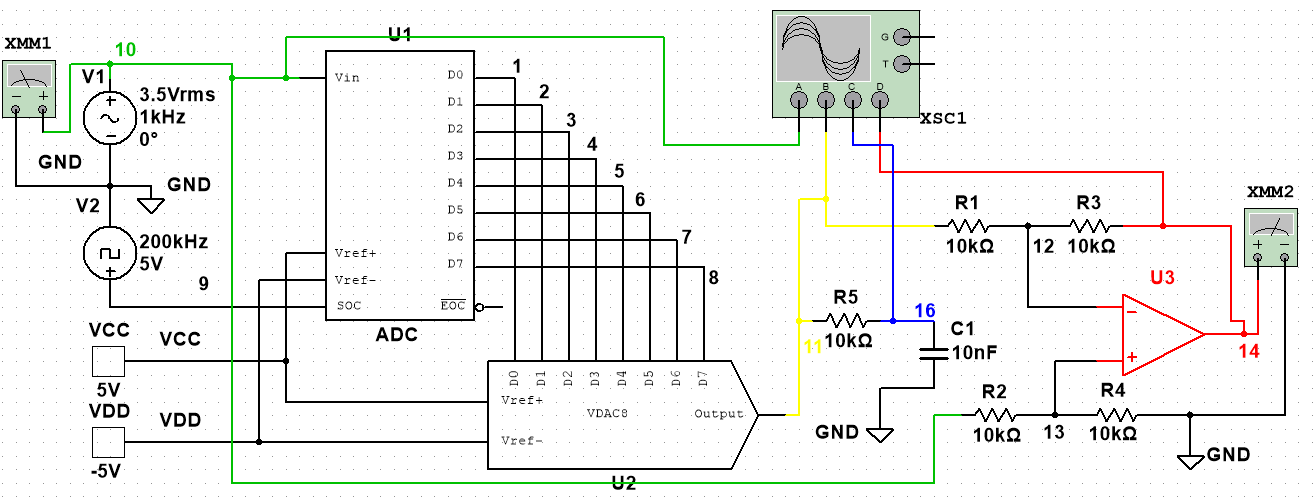
\includegraphics[width=0.9\textwidth]{schema.png}
    \caption{Simulační schéma}
    \label{schema}
\end{figure}

\section{Harmonické zkreslení}
Vzorkovací frekvence digitální domény byla nastavena na 10 kHz,
rozsah převodníku na interval [0, 5] V.
Simulace byla provedena pro frekvence vstupního signálu 1 a 15 kHz,
časové průběhy jsou srovnány na obrázku \ref{time-domain}.
Zeleně je vzorkovaný signál, žlutě je výstup DAC (uzel 11), modře je
výstup RC dolní propusti (uzel 16). Časová základna je \SI{200}{\micro\second}
na dílek a svislá osa má rozlišení \SI{5}{\volt} na dílek.

\begin{figure}[h]
    \begin{subfigure}{\textwidth}
        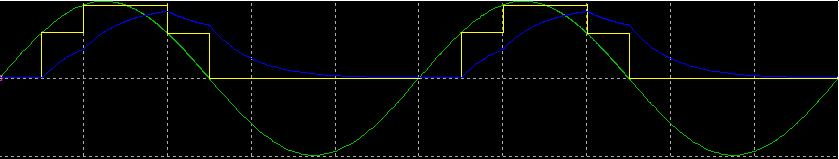
\includegraphics[width=\textwidth]{time-domain-1khz.png}
        \caption{Vstupní frekvence 1 kHz}
    \end{subfigure}

    \begin{subfigure}{\textwidth}
        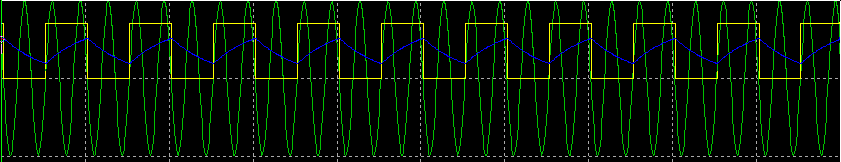
\includegraphics[width=\textwidth]{time-domain-15khz.png}
        \caption{Vstupní frekvence 15 kHz}
    \end{subfigure}
    \caption{Srovnání časových průběhů pro různé vstupní frekvence a fixní vzorkovací frekvenci 15 kHz}
    \label{time-domain}
\end{figure}

Pro obě frekvence byla provedena Fourierova analýza
po částech konstantního výstupu digitálně-analogového převodníku.
Spektra jsou srovnána na obrázku \ref{spektra}. Je vidět, že
kvůli aliasingu a zrcadlení ve spektru se frekvence signálu
15 kHz projevuje velkou špičkou na 5 kHz čáře.

\begin{figure}[h]
    \begin{subfigure}{\textwidth}
        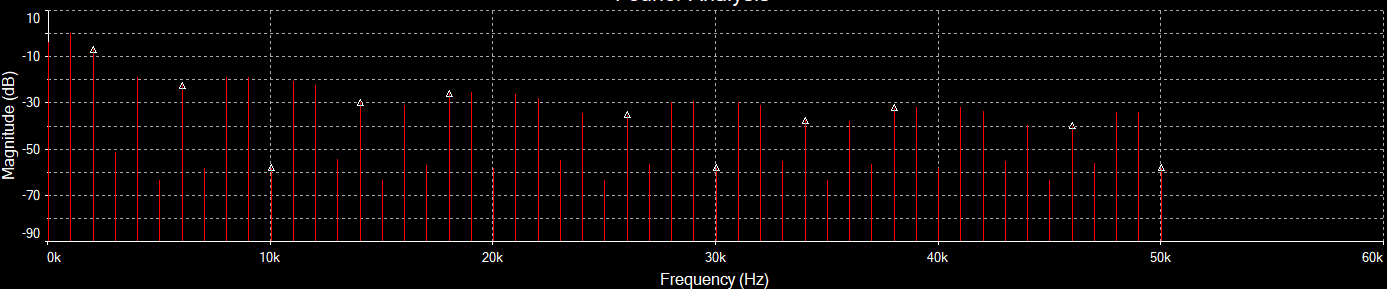
\includegraphics[width=\textwidth]{spektrum-1khz.png}
        \caption{Vstupní frekvence 1 kHz}
    \end{subfigure}

    \begin{subfigure}{\textwidth}
        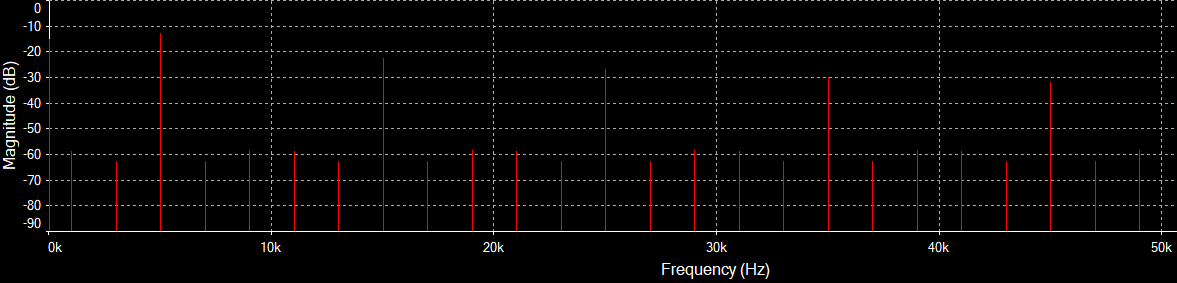
\includegraphics[width=\textwidth]{spektrum-15khz.png}
        \caption{Vstupní frekvence 15 kHz}
    \end{subfigure}
    \caption{Srovnání frekvenčních spekter signálů různých frekvence rekonstruovaných s asymetrickým rozsahem}
    \label{spektra}
\end{figure}

Činitele harmonického zkreslení THD -- spočtené pomocí vestavěné Fourierovy analýzy v Multisimu -- jsou vyneseny v tabulce \ref{thd}.

\begin{table}[h]
    \centering
    \begin{tabular}{c|c}
        vzorkovaná frekvence [kHz] & THD [\%]\\ \hline
        1 & 52.22 \\
        15 & 68.37 \\
    \end{tabular}
    \caption{THD v závislosti na frekvenci signálu pro 10 kHz vzorkování}
    \label{thd}
\end{table}

Pro srovnání byl převodníku nastaven symetrický rozsah vstupního napětí [-5, 5] V,
aby nedocházelo k ořezávání signálu. Tato úprava vedla na výrazně čistší spektrum
vykreslené na \ref{spektrum-sym} s THD pouze 15.2 \%.
Významný pokles je vidět ve velikosti stejnosměrné složky, která je rázem o 25 dB menší.
Na frekvenčním spektru je dobře pozorovatelná symetrie podle celočíselných násobků
vzorkovací frekvence 10 kHz.

\begin{figure}[h]
    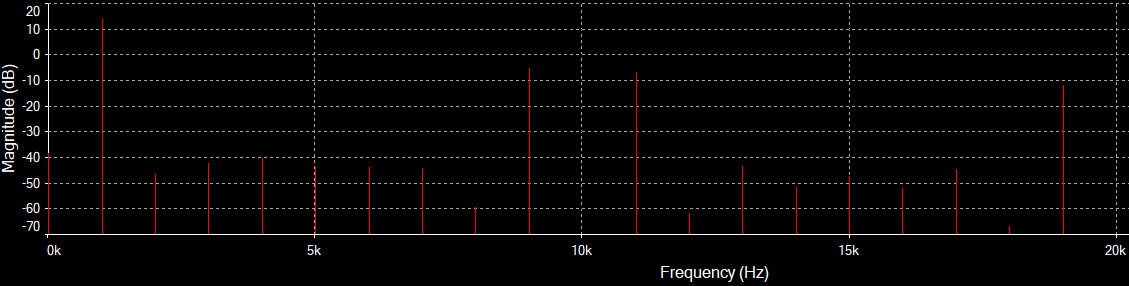
\includegraphics[width=\textwidth]{spektrum1-khz-sym.png}
    \caption{Spektrum rekonstruovaného signálu o frekvenci 1 kHz při vzorkování 10 kHz se symetrickým rozsahem}
    \label{spektrum-sym}
\end{figure}

\clearpage

\section{Kvantovací chyba}

S použitím vzorkovací frekvence 100 kHz a vstupního signálu o frekvenci 1 kHz
byla v uzlu 14 změřena efektivní hodnota
kvantovací chyby $U_{\rm q} = \SI{82}{\milli\volt}$ při efektivní hodnotě
signálu $U_{\rm sin} = \SI{3.5}{\volt}$. Tomu přísluší \textit{odstup signál-šum a zkreslení}
\begin{equation}
     SINAD = 20 \log \frac{U_{\rm sin}}{U_{\rm q}} = \SI{32.6}{\deci\bel}.
\end{equation}
\textit{Efektivní počet bitů} je
\begin{equation}
    ENOB = \frac{SINAD\text{(dB)} - 1.76}{6.02} = 5.12.
\end{equation}

\section{Zkreslení signálu vzorkováním}

Pro digitalizaci vstupního signálu $U_{in} = 3\sqrt{2} \sin \left(2\pi 1000 t\right)$ 
bylo vyzkoušeno
několik vzorkovacích frekvencí v rozsahu od 4 kHz do 128 kHz
v mocninách dvou kHz. Porování průběhů je na obrázkách \ref{srovnani-frekvenci}.
Originální signál je vykreslen zeleně, výstup DAC žlutě, vyfiltrovaný
rekonstruovaný signál modře, odchylka výstupu DAC od původního
signálu červeně. Časová základna je \SI{200}{\micro\second} na dílek,
na svislé ose mají všechny signály \SI{5}{\volt} na dílek
kromě červeného kanálu, jenž má pro lepší rozlišitelnost
 \SI{2}{\volt} na dílek.


\begin{figure}[h]
    \centering
    \begin{subfigure}{0.45\textwidth}
        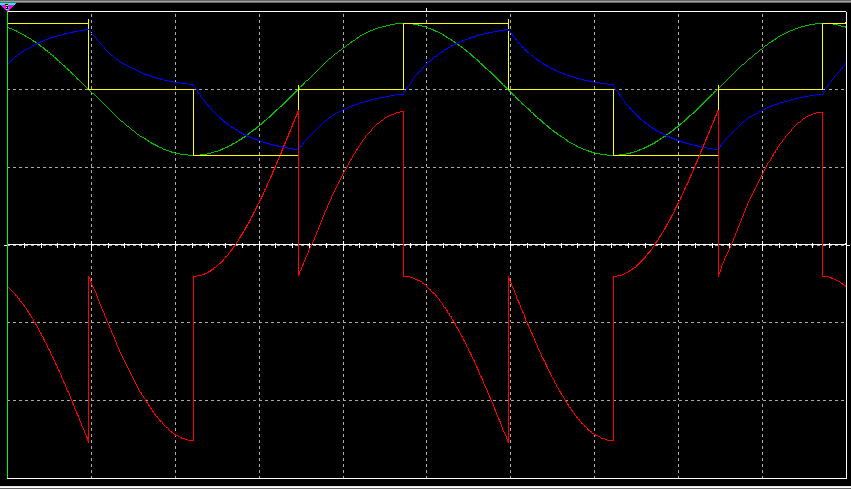
\includegraphics[width=\textwidth]{rekonstrukce-4kHz.png}
        \caption{Vzorkovací frekvence 4 kHz}
    \end{subfigure}
    \begin{subfigure}{0.45\textwidth}
        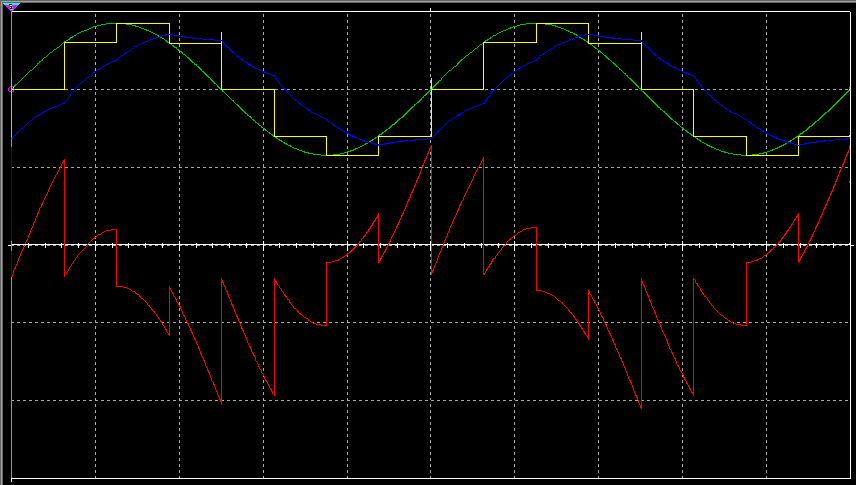
\includegraphics[width=\textwidth]{rekonstrukce-8kHz.png}
        \caption{Vzorkovací frekvence 8 kHz}
    \end{subfigure}

    \begin{subfigure}{0.45\textwidth}
        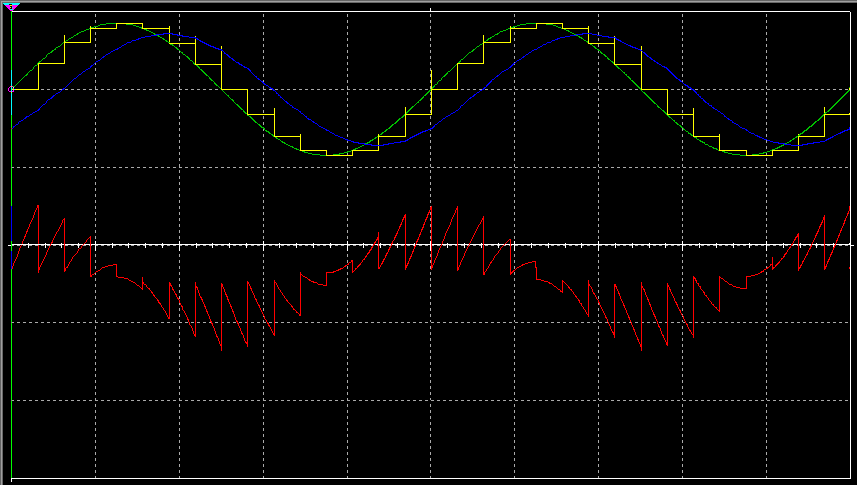
\includegraphics[width=\textwidth]{rekonstrukce-16kHz.png}
        \caption{Vzorkovací frekvence 16 kHz}
    \end{subfigure}
    \begin{subfigure}{0.45\textwidth}
        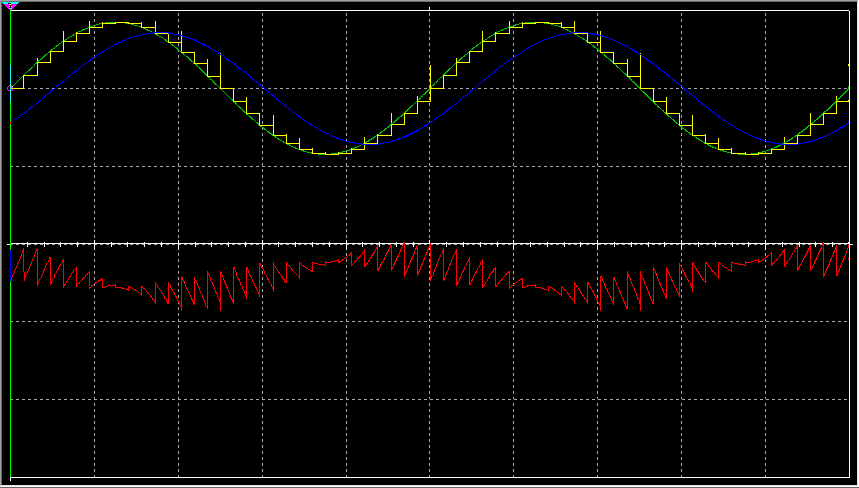
\includegraphics[width=\textwidth]{rekonstrukce-32kHz.png}
        \caption{Vzorkovací frekvence 32 kHz}
    \end{subfigure}

    \begin{subfigure}{0.45\textwidth}
        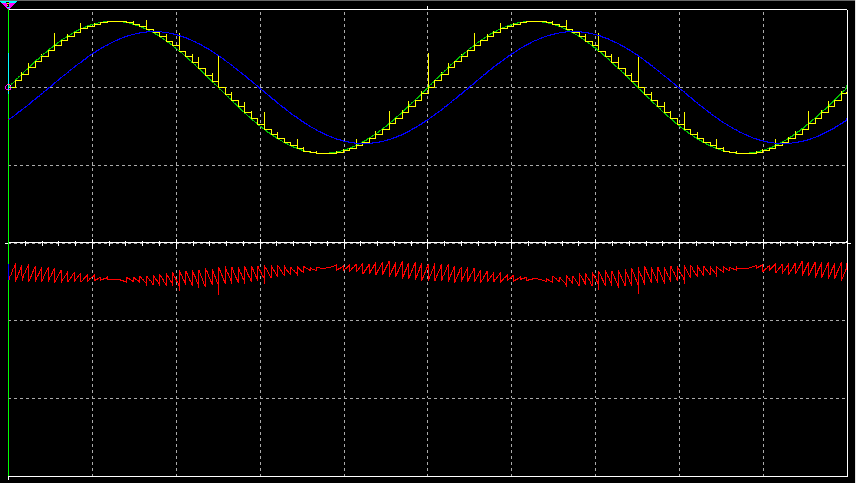
\includegraphics[width=\textwidth]{rekonstrukce-64kHz.png}
        \caption{Vzorkovací frekvence 64 kHz}
    \end{subfigure}
    \begin{subfigure}{0.45\textwidth}
        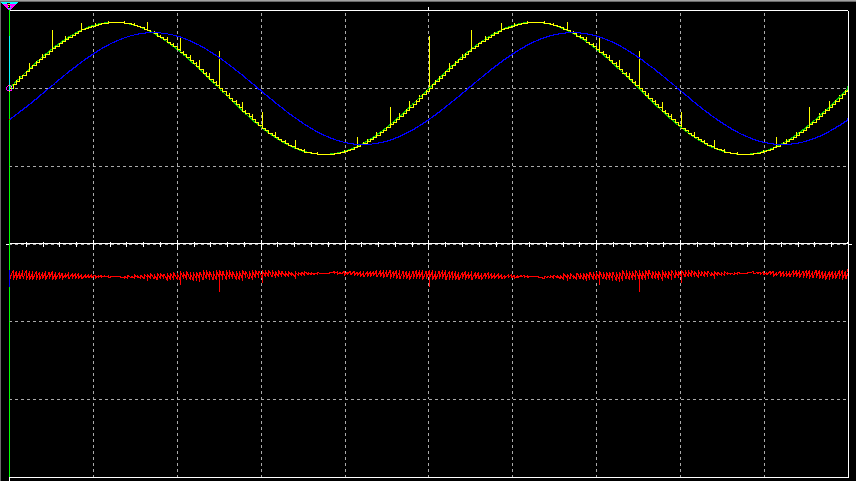
\includegraphics[width=\textwidth]{rekonstrukce-128kHz.png}
        \caption{Vzorkovací frekvence 128 kHz}
    \end{subfigure}
    \caption{Srovnání rekonstrukce signálu s různou vzorkovací frekvencí.}
    \label{srovnani-frekvenci}
\end{figure}

Ačkoli je vstupní signál pro všechny zvolené vzorkovací frekvence
rekonstruovatelný (je dodržen vzorkovací teorém),
u nejnižší použité frekvence 4 kHz je patrná amplituda chyby
až 4 V. Naopak pro frekvence 32 kHz a vyšší je velikost chyby omezená 
pod volt. Pro každou vzorkovací frekvenci byla změřena efektivní hodnota chyby
pomocí multimetru XMM2 ve schématu \ref{schema}. Naměřené efektivní hodnoty
jsou v tabulce \ref{chyby} a vykresleny na obrázku \ref{rms_chyba}

% Zpracováno s rms_chyba.m
\begin{table}
    \centering
    \begin{tabular}{c|c}
        vzorkovací frekvence [kHz] & RMS chyba [V]\\ \hline
        4 & 2.559 \\
        8 & 1.338 \\
        16 & 0.681 \\
        32 & 0.241 \\
        64 & 0.107 \\
        128 & 0.052        
    \end{tabular}
    \caption{Efektivní hodnota chyby v závislosti na vzorkovací frekvenci}
    \label{chyby}
\end{table}

\begin{figure}
    \centering
    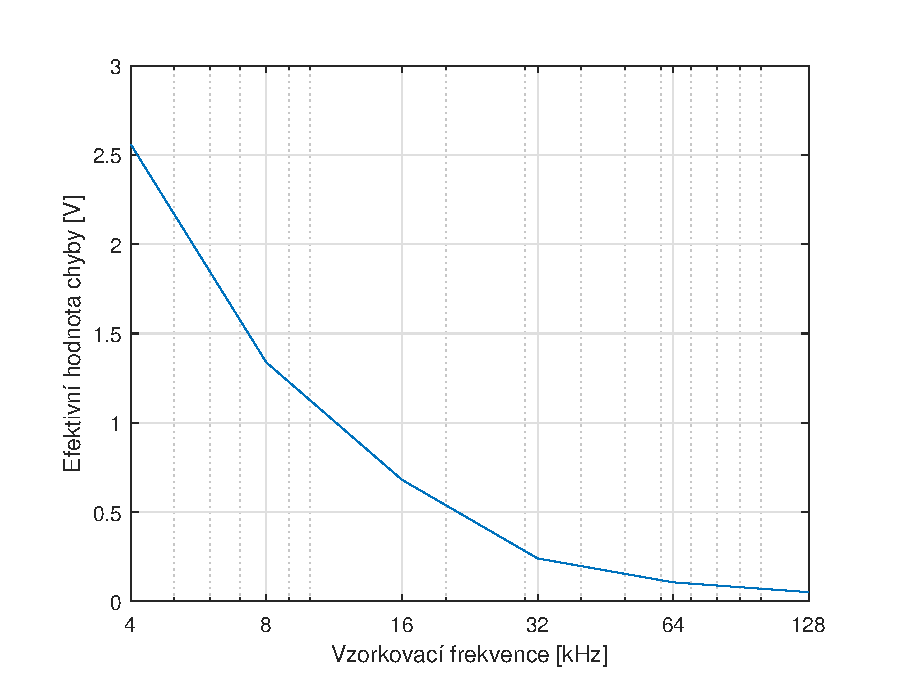
\includegraphics[width=0.6\textwidth]{rms_chyba.eps}
    \caption{Efektivní hodnota chyby v závislosti na vzorkovací frekvenci}
    \label{rms_chyba}
\end{figure}

\end{document}

